\documentclass[11pt,a4paper]{article}
\usepackage{ls}
\usepackage[main=english,german,russian]{babel}
\usepackage[utf8]{inputenc}
\usepackage{hyperref}
\usepackage{wrapfig}

\newenvironment{code}{\tt \begin{tabbing}
\hskip12pt\=\hskip12pt\=\hskip12pt\=\hskip12pt\=\hskip5cm\=\hskip5cm\=\kill}
{\end{tabbing}}
\def\dq{{\char34}}

\title{A Proposal for Modelling TRIZ System Evolution Concepts}

\author{Tom Strempel}

\date{Version of March 31, 2021}

\begin{document}
\maketitle

\section{Aim of the work}

The aim of this paper is to elaborate a proposal for an ontological modelling
of the areas of \emph{TRIZ System Evolution Concepts} based on the approaches
in \cite{TESE2018} and \cite{Shpakovsky2016} and further own investigations.
The work fits into the activities of the \emph{WUMM Ontology Project}
\cite{WUMM} to model core TRIZ concepts using modern semantic web means.  The
work consists of two parts -- a \emph{turtle file}, in which the semantic
modelling is performed based on the SKOS framework \cite{SKOS}, and \emph{this
  elaboration}, in which the backgrounds and motivations of the concrete
modelling decisions are detailed.

\section{Starting point} 

The central concern of practical TRIZ applications is the analysis, evaluation
and transformation of systems in order to improve their operational behaviour.
As in the lecture, the term transformation is understood in a broad sense and
also includes the planning and design of new systems as the transformation of
a system that is only available as vague conceptual requirements into a system
that operates in the real world. TRIZ provides a whole methodological toolbox
that can be used together with domain-specific concepts for the systematic
planning and implementation of such a transformation task. In the seminar we
observed that this TRIZ toolkit is embedded in broader reasoning contexts in
which engineering experience and scientific knowledge are systematised and
generalised.

One of the aspects examined in this context is the evolution of classes of
engineering systems in a historical context in order 
\begin{enumerate}
\item to extract repeating patterns of engineering procedures as «laws»
  \cite{Altshuller1979}, «laws, evolutionary lines and trends» \cite{KS} or
  just «engineering trends» \cite{TESE2018} or
\item to identify evolutionary connections in the unfolding of the history of
  technology \cite{Shpakovsky2016}.
\end{enumerate}

Exploring this aspect, the focus on the exact form of the transformation of a
single system described above was left and, in the style of \emph{distant
  reading}, a variety of information about historical transformations in
different classes of systems has to be analysed in order to extract
transformation patterns from it.  If, for example, the «development of
display» \cite[p. 22]{TESE2018}, \cite[ch. 5]{Shpakovsky2016} is analysed,
this is based on a much stronger abstraction of the system concept compared to
the system concept of classical TRIZ modelling, even if this more
comprehensive abstraction is only rarely explicated in the relevant works --
for example as a \emph{class of systems} in the narrower sense. In the rest of
this paper, the concept of system is used in the same vague generality of an
intuitive understanding as an externally given (metaphysical) concept as in
the referenced works, without attempting to go into more details.

The central to TRIZ understanding, that engineering achievements can be
conceptualised as system transformations, leads in the analysis of historical
technology development to the structure of a directed graph with the
prototypical link
\begin{center}\tt
  OldSystem \textrm{---}\fbox{isTransformedInto}$\to$ NewSystem
\end{center}
In the first approach, this graph is considered as a set of such links to be
classified. The graph structure plays a subordinate role, because even in the
concept of \emph{development line} a rather linear progression is postulated
(e.g. \cite[Figure 4.104]{KS}, but see \cite[4.8.4 and Figure 4.72]{KS}). In
the second approach \cite{Shpakovsky2016}, the graph structure is considered
more consistently, but also with the aim to classify the links in more detail.

The aim of these conceptualisations is on the one hand to develop the
methodology of \emph{evolutionary potential analysis} \cite[4.8.7]{KS} and on
the other hand to consolidate and improve the central TRIZ tools such as the
40 application standards («principles») or the 76 inventive standards.

\section{The Conceptualisations}

The conceptualisations to be developed follow the basic assumptions and
positings that are elaborated in more detail in \cite{Graebe2021}. In
particular, the following namespace prefixes are used:
\begin{itemize}[noitemsep]
\item \texttt{ex:} -- the namespace of a special system to be modelled. 
\item \texttt{tc:} -- the namespace of the TRIZ concepts (RDF subjects).
\item \texttt{od:} -- the namespace of WUMM's own concepts (RDF predicates,
  general concepts). 
\end{itemize}
Furthermore the \texttt{SKOS} ontology is used to model labels and definitions
of the object.

Our central task is to model the links in concrete evolutionary trees. The
full evolution tree as an edge-marked graph then can be conceptualised as a
set of such links in the usual way.

A link in such a concrete evolution graph has the typical shape
\begin{center}\tt
  ex:TVWithLargePixels ex:decreasePixelSize ex:TVWithMediumPixels .
\end{center}
where the transformation predicate \texttt{ex:decreasePixelSize} is assigned
to certain evolution patterns (even several).
\begin{code}\tt
ex:decreasePixelSize \\
\> a rdf:Property, skos:Concept ; \\
\> od:usesPattern tc:SegmentationPattern ; \\
\> skos:prefLabel "Decrease pixel size"@en ; \\
\> skos:definition """Decrease pixel size by segmentation \\
\>\> of one big pixel in several smaller ones"""@en .
\end{code}

\section{Concepts}

In this section the concepts developed by Shpakovsky in \cite{Shpakovsky2016}
are introduced and discussed.

\subsection{Structured information field}

There are three types of problems in modern engineering: the solution of
urgent technical problems, the forecast of the evolution of technical system
and patent protection or circumvention. While the importance of the first two
types are very easy to understand for non-engineers, the third type requires
some explanation. If a technical system is patented one must either pay the
owner of the patent or develop a competing system which is not covered by the
patent, both options are money and labor intensive. If such measures are not
taken a company risks to be sued out of contracts.

An example for that would be the ongoing case between Heckler \& Koch (HK) and
C. G. Haenel over the production of the new standard issue weapon of the
German army. The case is centered around the over-the-beach capability of the
weapon, which means that the weapon can still be fired after being submerged
in water for a short time. If the water is not removed the weapon can jam or
missfire. HK patented a solution for this problem in
\href{https://patents.google.com/patent/EP2018508B1/en}{EP2018508B1} by adding
a fluid passage to the recoil spring mechanism. HK argues that the system used
in the Haenel Mk556 is a violation of it's patent, while Haenel says it is
distinct from this patent. HK managed to kick Haenel out of the procurement
process with this argumentation. Haenel thus lost a big order because of a
(perceived) patent violation. This example illustrates very well why patent
protection and circumvention is an essential part of modern engineering.

Conventional solution methods such as trial and error and brainstorming are
not suited for the requirements of these three problems. A higher level
system, the \textit{science of invention}, must be created to adequately
tackle these problems. This system must obey the five requirements listed
below: 
\begin{enumerate}[noitemsep]
\item Objective classification criteria (objectiveness)
\item The presence of all significantly different versions (fullness)
\item Suitable degree of generalisation and specificity
\item Visualization (to find gaps for patent circumvention)
\item Sufficient description or prediction of not yet existing versions
  (informativity)
\end{enumerate}

In the following sections the concept of the evolution pattern and tree are
described which will fulfill these requirements.

\subsection{Evolution patterns and trees}
% scope is object, not the technical system

\begin{enumerate}[noitemsep]
\item Mono-Bi-Poly
\item Trimming
\item Expanding-trimming
\item Segmentation
\item Geometrical evolution
\item Object structure evolution
\item Evolution of surface properties
\item Dynamization
\item Increasing the controllability
\item Increasing the coordination of the elements
\end{enumerate}

From these ten basic evolution patterns, more specific evolution patterns can
be created. The evolution patterns from one to four are patterns that provide
resources for other evolution patterns. For example, there is no possibility
for dynamization on an unsegmented monolith. The structure of the object is
given by patterns five to seven. Patterns for dynamization, controllability,
and coordination are inserted at points that seem reasonable. This
hierarchical structure of transformations is shown in
Fig. \ref{fig:basic_evo}. It is not required to follow an evolution pattern to
its end before applying a different one. The direction of evolution is also
not strictly given. 

\begin{figure*}[htb]
  \centering
  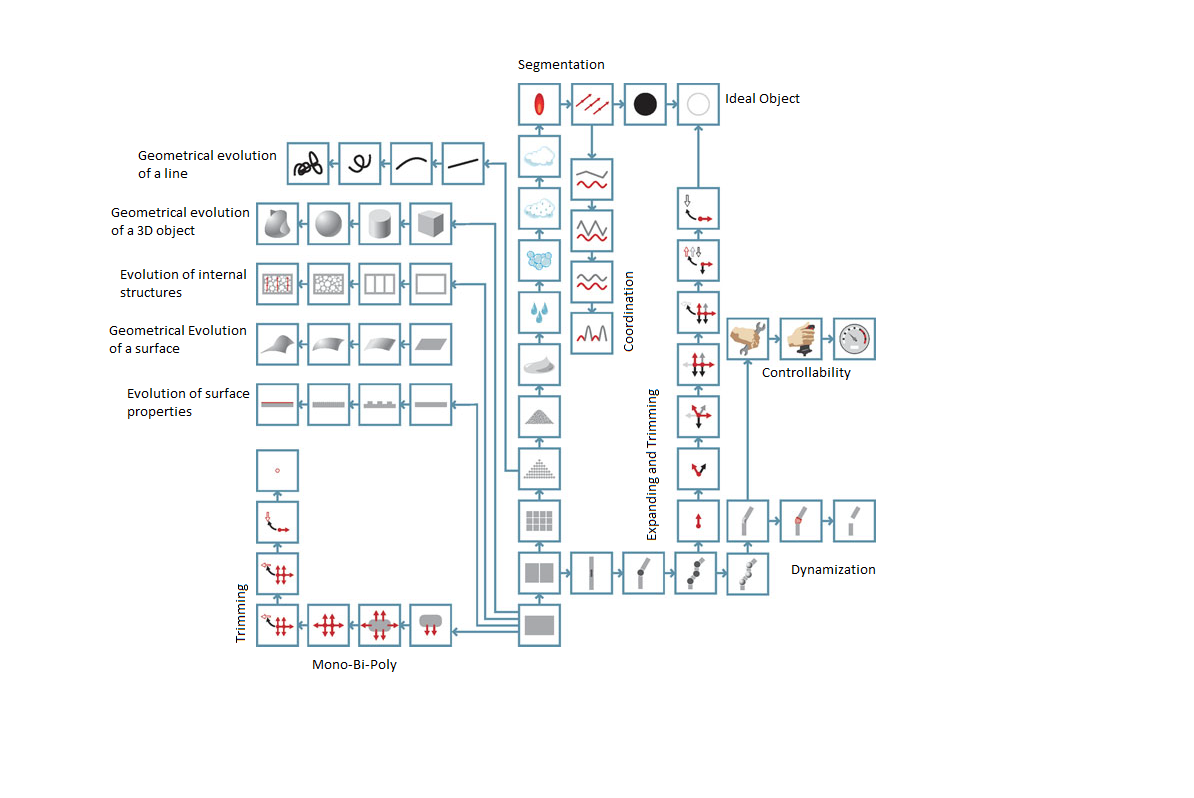
\includegraphics[width=\linewidth]{figures/basictree.png}
  \caption{\small Basic evolution tree \cite{Shpakovsky2016}}
  \label{fig:basic_evo}
\end{figure*}

A basic principle in TRIZ is the interaction of a tool and an (work) object:

\begin{center}\tt
  Tool \textrm{---}\fbox{interactsWith}$\to$ Object
\end{center}

Analogous to this a transformation is the application of an evolutionary
pattern to an object, which subsequently becomes a transformed version of the
object. Equivalents of these Patterns can be found in the TRIZ principles
e.g. the Segmentation Pattern corresponds to the first TRIZ principle
\textit{Principle of decomposition or segmentation}.

An evolution tree is build out of multiple patterns which are combined at
certain locations (see Fig. \ref{fig:basic_evo}). The positions of these
locations are specific for each specialized evolution tree and are only shown
in approximation here.

The Evolution Tree is a self-similar concept, e.g. an object is approximately
similar to itself. An Evolution tree can thus contain another evolution tree,
e.g. the evolution tree of the screen contains the evolution tree of a plasma
screen, which could be analysed further.

\subsection{Not laws but recommendations}

Shpakovsky never calls his concepts of the evolution pattern and tree laws but
uses the terms requirements, rules and, in context with construction
instructions, recommendations. Thereby he himself softens the objectivity of
his concepts. A really explicit explanation of this change from law to
recommendation does not take place, but the circumstance can be understood on
the basis of the created evolution tree of the screen.

The trunk of an evolutionary tree, for example, should consist of only one
evolutionary pattern (cf. \cite[p. 122f]{Shpakovsky2016}), but it becomes
clear that in the case of the screen two evolutionary patterns serve as the
trunk, namely trimming and segmentation. Here it is appropriate, due to the
nature of the object, not to follow the recommendation. This would not be
possible with a law or it should not occur at all due to the nature of a law.

\subsection{Outside influence}

The transition between some steps of evolution patterns require outside
development, e.g. the transition from a changeable image (flip-book cinema) to
the cinematographer was a joint product of many inventors. Outside involvement
is so required for adding and evolving objects e.g. in the mono-bi-poly,
segmentation and expanding-trimming pattern.

In a discussion with Shpakovsky it was clarified that this outside influence
can be seen as taking the same and new components from a super system, which
is outside the scope of the model. Components are selected on the basis of
their benefit in increasing productivity and other quality parameters. Outside
influence is not modelled in the RDF part.

\subsection{Construction of evolution trees}
% 2 Sachen: Welche Sachen nehme ich rein, und in welchem detaillierungsgrad

There are two question to answer before building an evolution tree: Which
objects should it include and in which level of detail are they included?
Context and a subsequent demarcation between the inside and outside of the
system is required. But the determination of the context is implicit or very
week by using the elemental function. Objectivity, rules and laws are only
applicable where the context can be adequately defined, which is not entirely
the case for the concept of evolution trees.

After an email correspondence with Shpakovsky the following conclusion for
creating a evolution tree was created:

After defining the elemental function, that should at best be dividable to the
\textit{subject-action-object} level, the simplest transformation of the
object is used as the starting point. Because the evolution tree is a self
similar concept the number of possible transitions and transformation versions
gets too big to keep track off. The inevitable limiting of this explosion of
versions follows a purely voluntary approach, as such objectivity can't be
guaranteed. The evolution tree does not touch either historical or temporal
rules. The sequence of options is subject only to technological trends. That
is, there is no goal of building a tree as such, or rather, the goal is to get
an information field in which the past, present and possible variants of the
system under analysis are located.

\subsection{Determination of not known versions}

\begin{figure}[htb]
  \centering
  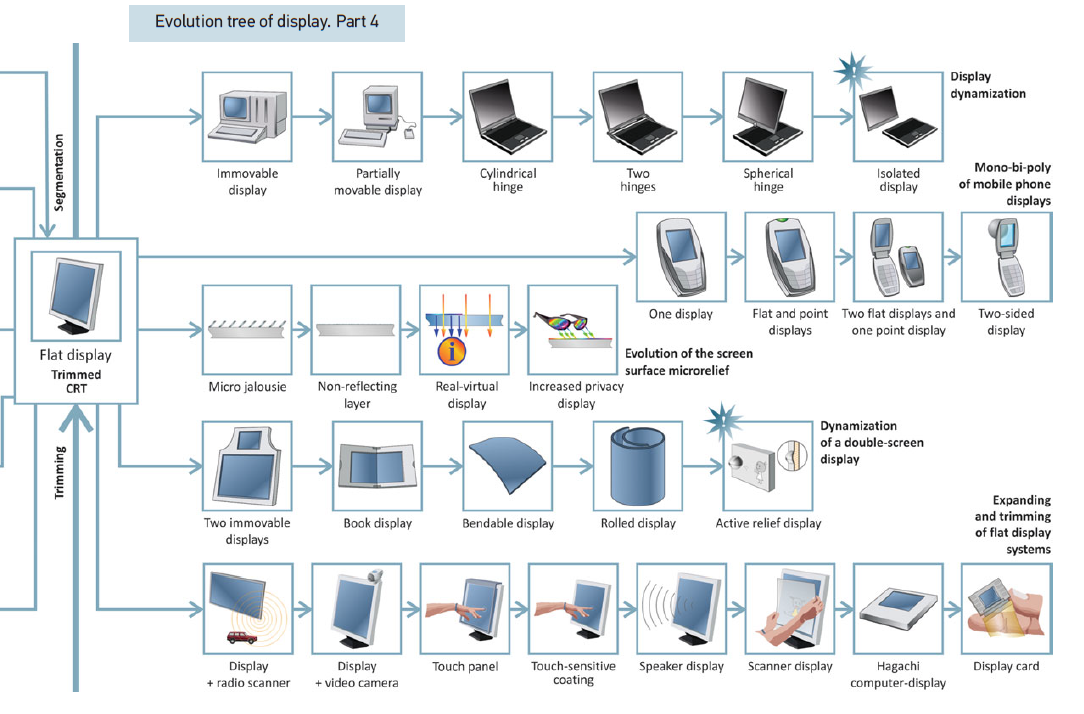
\includegraphics[width=.9\linewidth]{figures/removabledisplay.png}
  
  \caption{\small Section of the specific evolution tree of the screen
    \cite{Shpakovsky2016}, see \url{http://www.target-invention.com/} for
    the complete tree}
	\label{fig:spec_evo}
\end{figure}

For the analysis of an object, both the basic (see Fig. \ref{fig:basic_evo})
and the specific evolution tree (see Fig. \ref{fig:spec_evo}) must be created.
By comparing the two trees, gaps as well as unfinished evolutionary patterns
can be discovered. The highest level of the pattern of dynamization consists
of a complete decoupling of the individual components. For a laptop, this
would mean separating the screen and peripherals. At the time the evolutionary
tree of the screen was created around 2002, this version of the object did not
yet exist. By recognizing this gap, a useful new version was found. Nowadays,
complete dynamization is achieved by integrating the computing technology into
the screen and connecting the peripherals via Bluetooth. Thus it was shown
that evolution trees are able to map future developments.

\subsection{Patent circumvention}

There is often the problem that a patent already exists for a desired
product. In this situation it is either possible to pay high license fees to
the patent owner or to circumvent the patent.

The legal method of patent circumvention, which consists of using loopholes
and erroneous patent descriptions to invalidate a patent, is not always
applicable.

It is alternatively possible to modify the object under investigation to
develop a better product. This inventive method has the disadvantage of having
large development costs and having to change the basic design. On the other
hand, it is not possible to obtain an alternative patent without modification.

From this conflict, typical for TRIZ, a synthesis emerges in the form of the
legal-inventive method. This new method aims at finding transformation
versions not yet covered by patents through evolution trees.

The search for existing patents can be additionally facilitated by using the
object and transformation names as keywords.  

But as seen in the example case between HK and Haenel this is not a hundred
percent secure protection. Even not yet clarified legal uncertainties can lead
to not getting the desired contract, because the contractor doesn't want to
take the risk or is legally not allowed to due to the ongoing case. 

\section{Modelling}

Ontologies are based on the modelling on models. This is done over several
levels, where the lower levels are used to model real-world examples and thus
have a high level of specificity. Higher levels are used to model concepts and
even more general concepts. In this work three levels are used for modelling
which results in three RDF namespaces: 

\begin{itemize}[noitemsep]
\item \texttt{ex:} -- Level 1 (Real world examples and patterns)
\item \texttt{tc:} -- Level 2 (Subjects and concepts)
\item \texttt{od:} -- Level 3 (Predicates) 
\end{itemize}

\subsection{Modelling the evolution tree concepts}

File \textit{EvolutionTree.ttl} contains the description for the concepts for
evolution trees presented in \cite{Shpakovsky2016}. It also contains all
modelled basic evolution patterns and thus the basic evolution tree.

All RDF subjects or nodes in the corresponding graph are part of the
\texttt{tc:} namespace. New predicates in \texttt{od:} didn't need to be
modelled because the already existing ones covered every need. Every chapter
and subsection in the table of contests is modelled with at least one subject
or triple, e.g. the segmentation pattern has it's own RDF subject
\texttt{tc:SegmentationPattern} and is described in it.


\begin{code}\tt
tc:SegmentationPattern \\
\> od:subConceptOf tc:BasicEvolutionPattern ; \\
\> od:hasSubConcept tc:Monolith, tc:TwoParts, tc:ManyParts, tc:Granules, \\
\> tc:Powder, tc:Paste, tc:Liquid, tc:Foam, tc:Fog, tc:Gas, tc:Plasma, \\
\> tc:Field, tc:Vacuum, tc:IdealObject ; \\
\> a skos:Concept, od:AdditionalConcept ; \\
\> skos:prefLabel "Segmenting objects and substances"@en ; \\
\> skos:example "Segmentation of an aircraft propulsion unit"@en ; \\
\> skos:broader tc:Segmentation, tc:TrendofTransitiontoMicrolevel .
\end{code}
\begin{code}\tt
tc:Liquid \\
\> od:subConceptOf tc:SegmentationPattern ; \\
\> a skos:Concept, od:AdditionalConcept ; \\
\> skos:prefLabel "Liquid"@en . \\
\end{code}

Relations or edges between subjects are modelled by the predicates
\texttt{od:subConceptOf} and \texttt{od:hasSubConcept}, e.g. as
\texttt{tc:SegmentationPattern} is a \texttt{tc:BasicEvolutionPattern} there
are linked together. Different transformation versions like
\texttt{tc:Monolith} are also referenced that way.

Transitions of a generic evolution pattern like \texttt{tc:FlatSurface} to
\texttt{tc:CylindricalSurface} from \texttt{tc:GeometricalEvolutionPattern}
are not modelled as the direction could be both ways in an specific
example. Some modern monitors use curved displays instead of flat ones. CRT
displays have a cylindrical surface due to constrains in manufacturing. By
using better glass it is possible to get a CRT display with a flat
surface. With that a conflict would arise if the evolution is only possible in
one direction. Shpakovsky also introduces the MATChEM-Operator from the wider
TRIZ as a not-listed extra pattern.

As TRIZ trends are used as the basic evolution patterns they must be
referenced from the modelled patterns, e.g. \texttt{tc:Segmentation} and
\texttt{tc:TrendofTransitiontoMicrolevel} are referenced by
\texttt{tc:SegmentationPattern} via \texttt{skos:broader}. Evolution pattern
are more specific than their corresponding TRIZ principles because they are
seen in the context of the evolution tree and thereby \texttt{skos:broader} is
used instead of \texttt{skos:narrower}.  

\begin{code}\tt
tc:Segmentation \\
\> od:hasRecommendation tc:Segmentation\_1, tc:Segmentation\_2,\\\>\>
tc:Segmentation\_3 ; \\ 
\> od:hasAltshuller73Id "01" ; \\
\> od:hasAltshuller84Id "01" ; \\
\> a od:Principle ; \\
\> rdfs:label "Principle of decomposition or segmentation"@en .
\end{code}

Triples usually consist of the RDF subject (TRIZ concept), the referenced
subjects via predicates, the \texttt{a} predicate, and further skos labels,
examples and definitions. All information about one subject is modelled inside
a single triple. The file also contains comments marked with \texttt{\#} where
the currently modelled part is marked or further described to keep track. 

Concepts for the application of the evolution trees are also modelled via
subconcepts and the skos ontology: 
\begin{code}\tt
tc:FrontalSearch \\
\> od:subConceptOf tc:InformationFieldSearch ; \\
\> a skos:Concept, od:AdditionalConcept ; \\
\> skos:prefLabel "Frontal search of an Information Field"@en ; \\
\> skos:definition """Search starts from random points. \\
\>\> Search of the whole information field for relevant information."""@en .
\end{code}

\subsection{Modelling the screen evolution tree}

Shpakosvky modelled the evolution tree of the screen with \textit{To visualize
  information} as the elemental function. We see a display in this context as
an \textit{artificially created object specially designed for the role of a
  tool in the realization of the elemental function}\cite{Shpakovsky2016} to
differentiate it from a sheet of paper with information written on it. The
terms display and screen are used interchangeably in this work. The main axis
of development runs along the trimming transition between the cinematographer,
trimmed cinematographer, CRT TV set and the flat display. Further transitions
are part of the segmentation pattern. The evolution tree trunk is marked by
using \texttt{od:usesPattern tc:EvolutionTreeTrunk} in the
transitions. \texttt{ex:} is used as the namespace of subjects and predicates
for the model because it describes an real world example. As the granularity
of this specific evolution tree is very fine some predicates or transitions
can be used multiple times for transforming subjects.

First off the screen will be defined as an specific evolution tree:
\begin{code}\tt
ex:Screen \\
\> a tc:SpecificEvolutionTree ; \\
\>\> skos:prefLabel "Specific evolution tree of the screen"@en ;
\end{code}

\begin{figure}[htb]
  \centering
  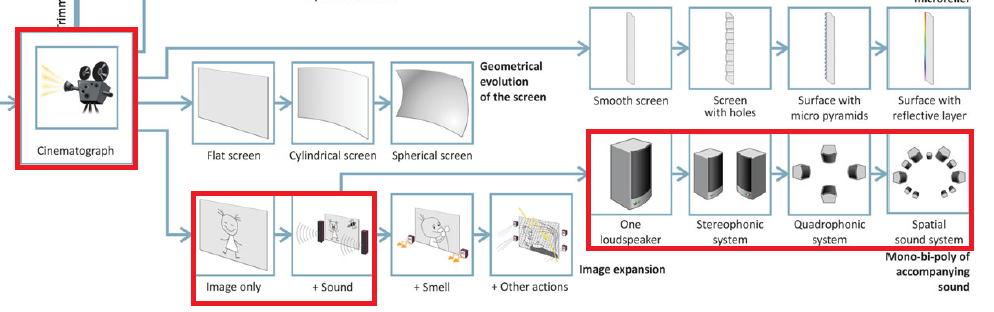
\includegraphics[width=.9\linewidth]{figures/audio.png}
  \caption{\small Pattern of adding audio \cite{Shpakovsky2016}}
  \label{fig:audio}
\end{figure}

We will using the marked transformations for adding sound to the screen (see
Fig. \ref{fig:audio}) as an example for the structure of the modelling done in
\textit{ScreenExample.ttl}.

\begin{code}\tt
ex:Cinematograph \\
\> a ex:Screen ; \\
\> ex:transitionsTo ex:ImageOnly, ex:FlatScreen, ex:SmoothScreen,\\\>\>
ex:ImmovableScreen ;\\ 
\> ex:trimCinemaBuilding ex:MechanicalTVSet ;\\
\> skos:prefLabel "Cinematograph"@en .
\end{code}

We choose the cinematographer from the evolution tree trunk as the starting
point of our example. Fig. \ref{fig:audio} shows that different objects that
are part of the cinematographer can be branched out and be described. No
transformation needs to take place because we only look at an already existing
object. For this purpose the \texttt{ex:transitionsTo} predicate is used as it
describes a transition without changing the object. This leads to
\texttt{ex:ImageOnly} to which we add sound via the \texttt{ex:addSound}
transition. \texttt{tc:MonoBiPolyPattern} and \texttt{tc:BiSystem} are used as
the types of the transitions because components are added to build a higher
level system. Where applicable the concrete step of the evolution pattern
(e.g. \texttt{tc:BiSystem}) is used, if not only the basis evolution pattern
(e.g. \texttt{tc:MonoBiPolyPattern}) is used. 

\begin{code}\tt
\# Image expansion\\[4pt]
ex:ImageOnly\\
\> a ex:Screen ;\\
\> ex:addSound ex:ImageSound ;\\
\> skos:prefLabel "Image only"@en .\\[4pt]
ex:ImageSound \\
\> a ex:Screen ; \\
\> ex:addSmell ex:ImageSoundSmell ;\\
\> ex:transitionsTo ex:OneLoudspeaker ;\\
\> skos:prefLabel "Image and sound"@en .\\[4pt]
\# ...\\[4pt]
ex:addSound\\
\> a rdf:Property, skos:Concept ;\\
\> od:usesPattern tc:MonoBiPolyPattern, tc:BiSystem ;\\
\> skos:prefLabel "Add sound"@en .
\end{code}

Now we are in the mono-bi-poly pattern of accompanying sound in which the
predicate \texttt{ex:addLoudspeaker} is used to repeatedly add new
loudspeakers to the system to evolve it into a poly-system. This new
poly-system is of higher complexity due to higher coordination between the
loudspeakers by for example the Dolby Surround 7.1 specification. Using the
same transition repeatedly is not always possible. 

\begin{code}
\# Mono-Bi-Poly of accompanying sound\\[4pt]
ex:OneLoudspeaker \\
\> a ex:Screen ;\\
\> ex:addLoudspeaker ex:StereophonicSystem ;\\
\> skos:prefLabel "One loudspeaker"@en .\\[4pt]
ex:StereophonicSystem \\
\> a ex:Screen ; \\
\> ex:addLoudspeaker ex:QuadrophonicSystem ;\\
\> skos:prefLabel "Stereophonic system "@en .\\[4pt]
ex:QuadrophonicSystem \\
\> a ex:Screen ; \\
\> ex:addLoudspeaker ex:SpatialSoundSystem ;\\
\> skos:prefLabel "Quadrophonic system"@en .\\[4pt]
ex:SpatialSoundSystem\\
\> a ex:Screen ; \\
\> skos:prefLabel "Spatial sound system"@en .
\end{code}
\newpage
\begin{code}
ex:addLoudspeaker\\
\> a rdf:Property, skos:Concept ;\\
\> od:usesPattern tc:MonoBiPolyPattern, tc:BiSystem, tc:PolySystem ;\\
\> skos:prefLabel "Add loudspeaker"@en ;\\
\> skos:definition "Add one or more loudspeakers"@en .
\end{code}

\begin{wrapfigure}[26]{l}{0.4\textwidth}
  \begin{center}\vspace*{-1em}
    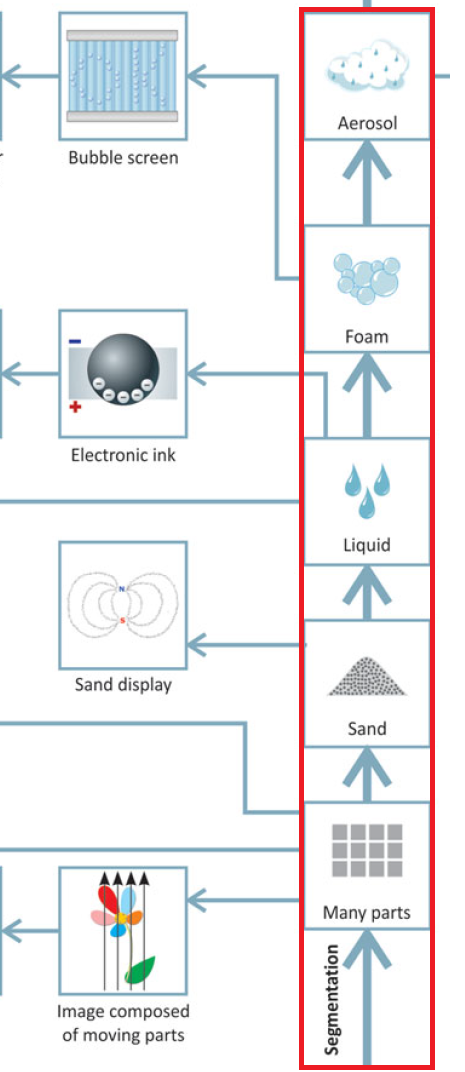
\includegraphics[width=0.3\textwidth]{figures/segmentation.png}
  \end{center}
  \caption{\small Segmentation of the screen \cite{Shpakovsky2016}}
  \label{fig:segmentation}
\end{wrapfigure}

With that we successfully modelled a branch of the evolution tree of the
screen, the same approach to modelling is used to completely model the tree.
One particularity must be explained further namely the further segmentation of
the screen shown in Fig. \ref{fig:segmentation}. Shpakovsky uses the generic
evolution transformations here even if it is a specific evolution tree. This
was modelled by using extra subjects (\texttt{ex:ManyParts}, \texttt{ex:Sand}
etc.) and linking them with the \texttt{ex:segmentation} predicate. Branches
are transitioned to with \texttt{tc:transitionsTo} as was explained before.

% a tc:SpecificEvolutionTree

\subsection{Modelling the ship propulsion evolution tree}

Souchkov in \cite{KS} describes the evolution tree using the example of the
boat. The terms boat and ship are used interchangeably here even if a ship is
assumed to have some other characteristics as a boat, e.g. being ocean-going
and having a higher displacement. 

This is done via the standard TRIZ methodology and can be implemented in
Shpakovsky's more specific concept of an evolution tree (see
\textit{BoatExample.ttl}). A boat as a technical system has a very wide array
of transformations. Thus it is vital to specify the elemental function by
looking at the main axis of the evolution, the tree trunk.

Souchkov splits the transformations into three categories: New transformations
for delivering the main function, existing transformations that could be
developed further and completed or discontinued transformations. We are
interested in the new transformations for delivering the main function as this
is used as the main axis of development. Developments follows through the
transformations tree trunk, rowboat, sailboat, steamboat, diesel-boat,
water-jetboat and atom-boat. Hence the corresponding elemental function is
\textit{provide the boat with a power source} as they all, with one exception,
describe what the engine or power source is. A tree trunk has no power source,
a rowboat uses muscle power, a sailboat the wind, a steamboat a steam machine
and so on. As the water-jet is a means of propulsion and does not describe the
power source, but how the power is used for propulsion (e.g. propeller, paddle
wheel), it is misplaced on the evolution tree trunk.
\newpage

Modelling this discrepancy is done via using a different evolution pattern for
the transition between the diesel-boat and water-jet-boat, namely the
expanding-trimming pattern. Consequently the transition is not part of the
modelled evolution tree, while all other transitions between the main
transformations are. 

The granularity of this tree is very coarse. The transitions between the main
versions e.g. from sailboat to steamboat are very big steps in the overall
technical development. First ships with sails were developed in the 2nd
millennium BCE in the South China Sea, while the first practical steamers were
build in the early 19th century, this massive time frame shows that the tree
is very coarsely build. Because of that transitions or predicates are very
specific as they must depict large developments. Finer grained evolution trees
have the advantage of reusing predicates, this is not applicable here. Again
we are running into the self similarity of the evolution tree as one tree node
could be easily expanded, e.g. the torpedo boat node could be expanded to
include all development on torpedo boats. Furthermore hybrid vessels
e.g. boats with stream and sail propulsion are also omitted. The terms boat
and ship are used interchangeably in the evolution tree and this approach was
further adopted. Predicates can possibly only applied for this example and
thus not be easily used for other objects. The branching transformations can
also be seen as evolution trees themselves as they describe extended elemental
functions like \textit{transporting tourists via boat}. 

There are two possibilities of modelling the evolution tree trunk, on one hand
the segmentation pattern can be used on the other the MATChEM operator, both
must describe the power source of the ship. If the segmentation pattern is
used the manual labour of rowing a boat with one or multiple rowers could be
described with the monolithic, two-part and many-part transformations. Because
a tree trunk has no on board power source of propulsion it would be omitted
from the evolution tree trunk. Sails use wind and thus gas for propulsion, so
no problems would arise here. Diesel engines burn a diesel air mix and direct
drive the propulsion device via a transmission, it would be thus modelled as a
liquid or aerosol. This is not the case for a steam engine or nuclear reactor,
they use boilers or reactors to boil water into steam and then drive a stream
engine or turbine. This would mean that three types of power sources would be
modelled with gas, which is not ideal. If we would model the fuel instead
other problems would arise because a boiler can burn coal (e.g. a many-parts
transformation), oil (e.g. the liquid transformation) or an coal-oil
mixture. Furthermore would a sailboat be on a higher place in the segmentation
pattern as the diesel engine. While it could be argued that the ideality of
using wind is higher, because no fuel needs to be burned, the cost of
executing it's function is still high as a lot of complex rigging, sails and
high manpower is required. 

\begin{figure*}[htb]
  \centering
  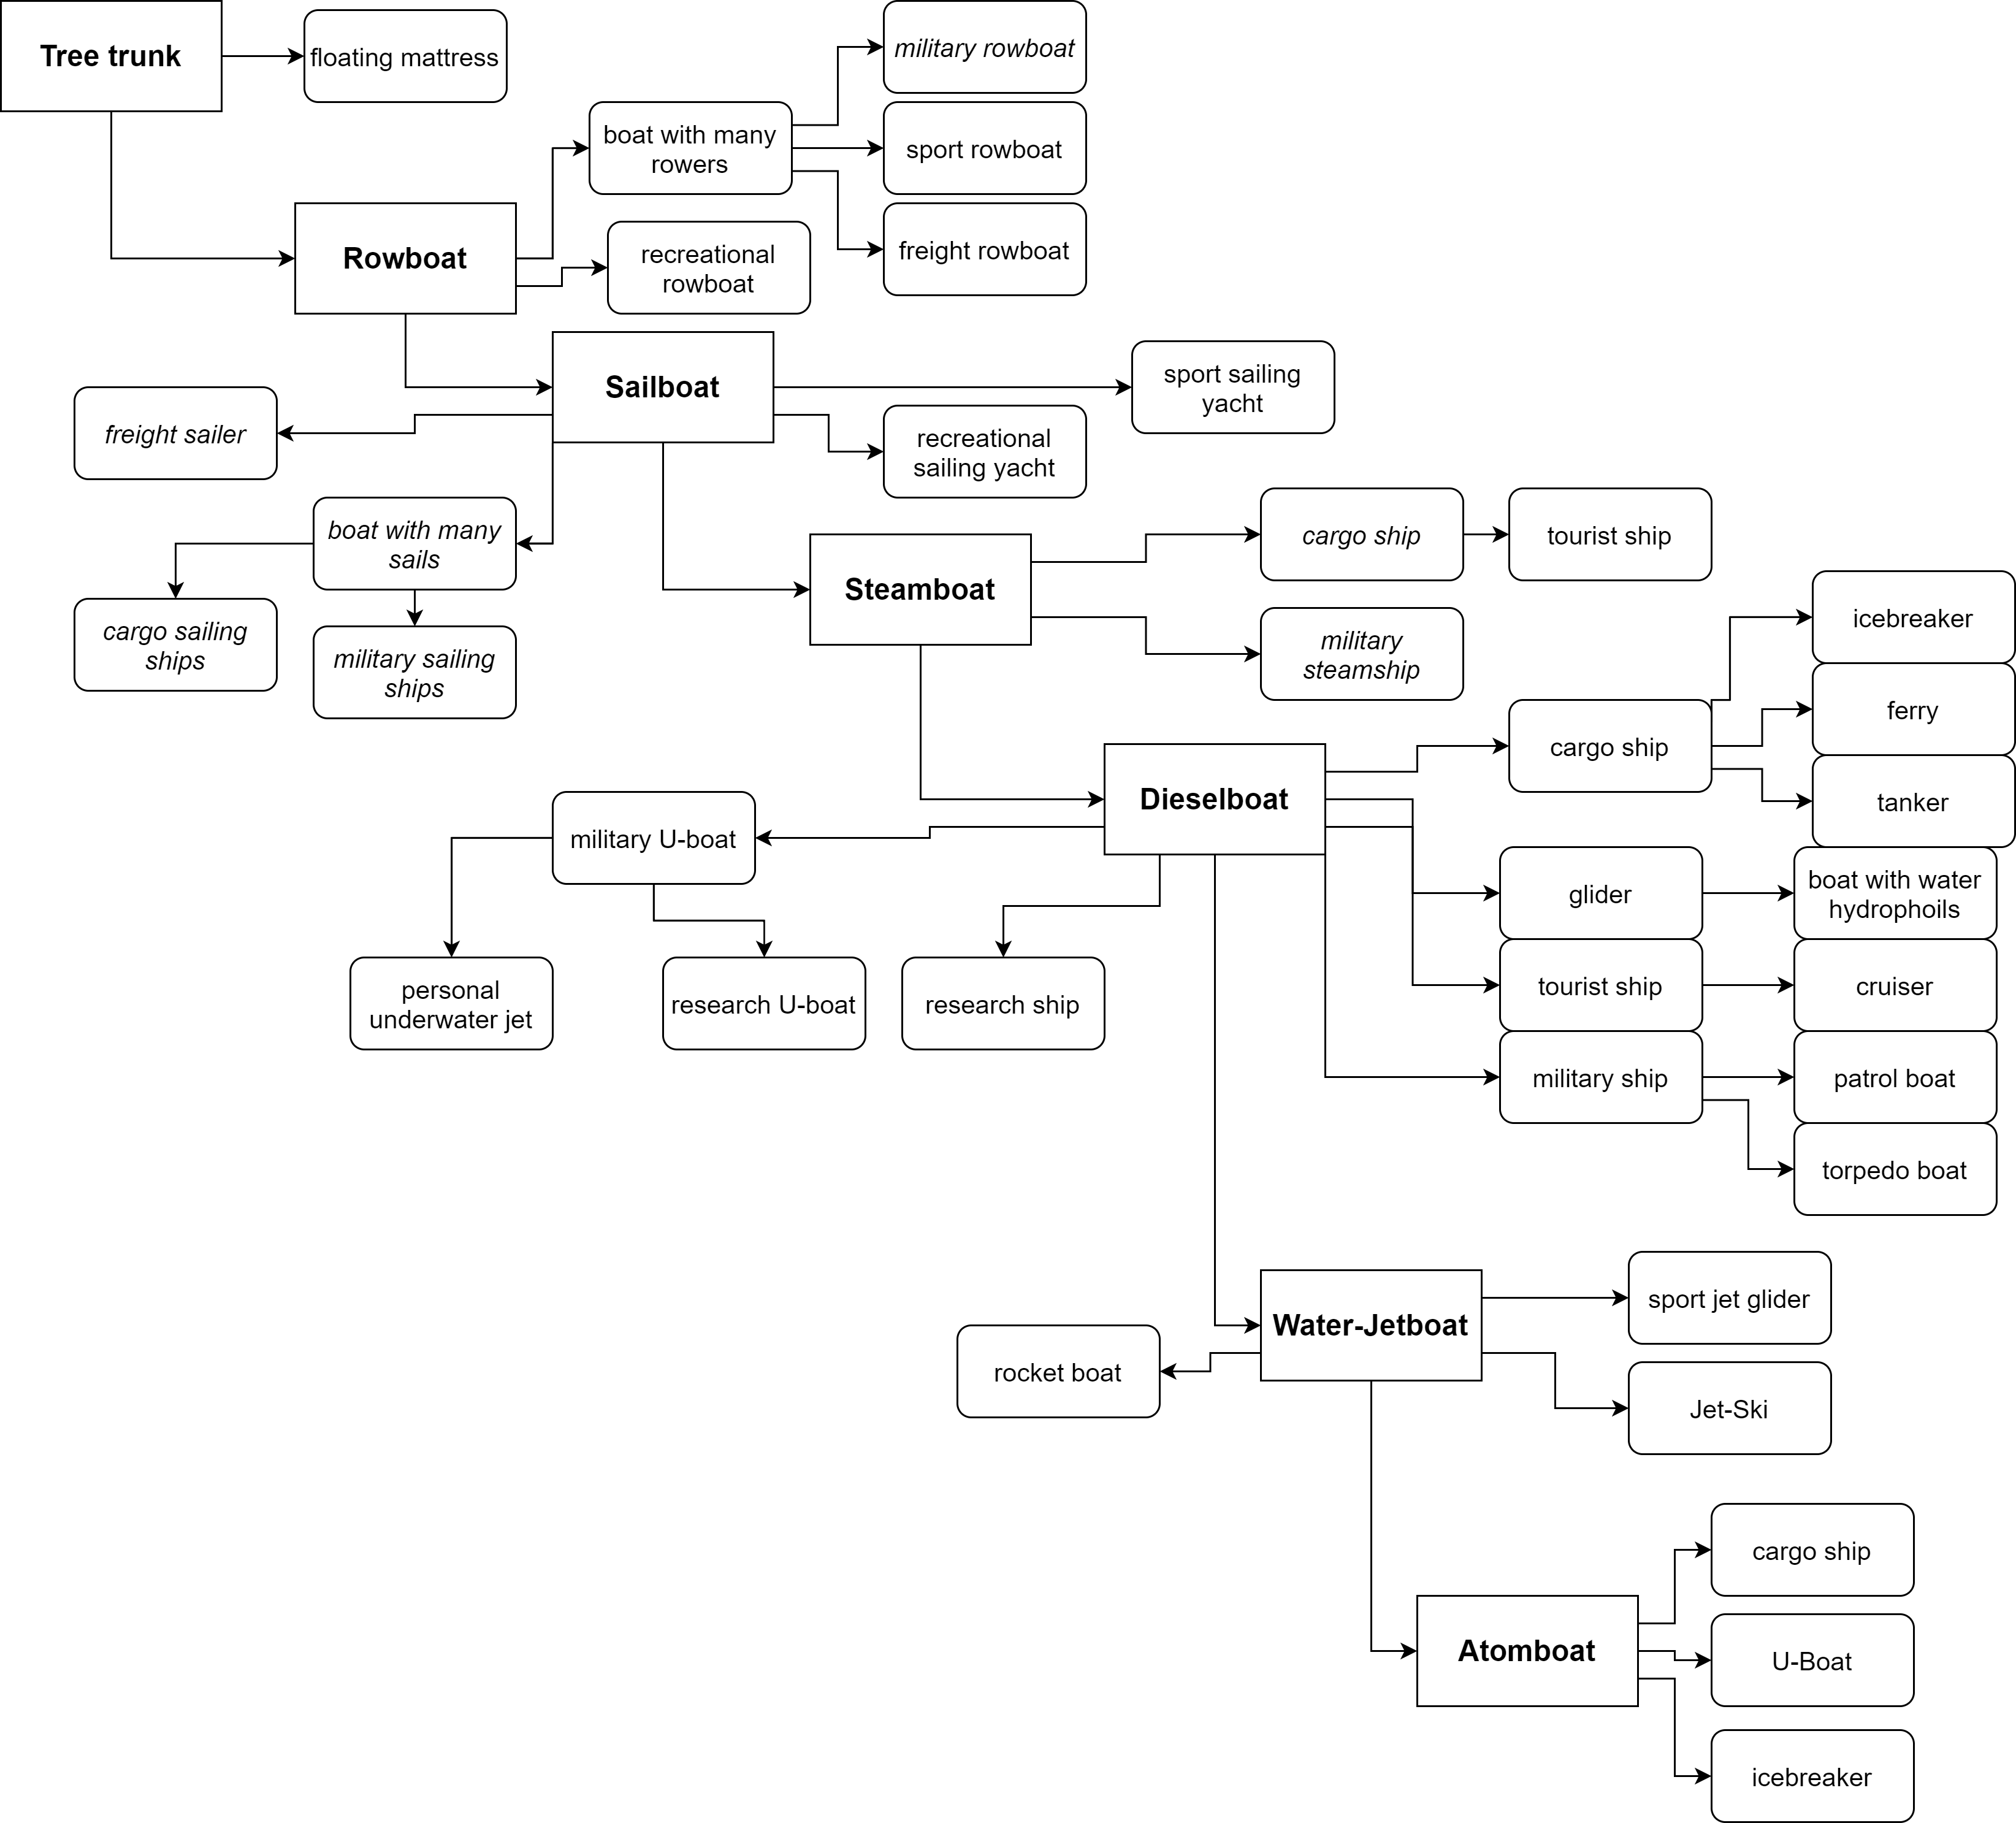
\includegraphics[width=\linewidth]{figures/boat.png}
  \caption{\small Souchkov's evolution tree of the boat translated from German
    \cite{KS}}
	\label{fig:boat}
\end{figure*}
\begin{tabular}{r@{: }l}
\textbf{Bold font} & new transformations for delivering the main function\\
Normal font & transformations that can be developed further\\
\textit{Italic font} & discontinued transformations
\end{tabular}

\begin{code}\tt
ex:Boat \\
\> a tc:SpecificEvolutionTree ; \\
\> skos:prefLabel "Boat"@en, "Boot"@de ; \\
\> skos:altLabel "Power source of the boat", \\
\>\> "Energiequelle bzw. Motor des Boots" ; \\
\> skos:definition "Specific evolution tree of the boat power source"@en . \\
\end{code}

Due to these problems a modified MATChEM operator will be used. This operator
is used for remodelling the technical system around different fields so that
their working principle is entirely different but their function remains the
same. For our fields we are using mechanical, air, thermal, chemical,
electrical and atomic fields. These model the evolution steps better and in
the right progression. The electric motor is omitted in the model but was used
with U-boats together with a diesel engine.

\begin{code}
ex:BoatMATChEMOperator\\
\> a tc:SpecificEvolutionPattern, tc:MATChEMOperator ;\\
\> skos:prefLabel "Use a boat specific MATChEM operator"@en ;\\
\> skos:definition """Mechanical - Muscle power\\
\> Air - Wind power via sail\\
\> Thermal - Steam engine\\
\> Chemical - Diesel engine\\
\> Electrical - Electric motor\\
\> Atomic - Nuclear fission reactor"""@en .\\[4pt]
ex:Rowboat \\
\> a ex:Boat ; \\ 
\> ex:addPaddles ex:BoatWithManyRowers ; \\
\> ex:addRecreationalInstallations ex:RecreationalRowboat ; \\
\> ex:replacePaddleWithSail ex:Sailboat ; \\
\> skos:prefLabel "Rowboat"@en ; \\
\> skos:definition "Manual labour as the power source"@en . \\[4pt]
ex:replacePaddleWithSail \\
\> a rdf:Property, skos:Concept ; \\
\> od:usesPattern tc:SegmentationPattern, tc:Gas ; \\
\> skos:prefLabel "Replace Paddle with sail"@en ; \\
\> skos:definition """Rudder and thus muscle power is replaced by sails \\
\>\> and thus wind power"""@en .
    
\end{code}

The transformations that can be developed further can be described as
incomplete evolution patterns. The expanding-trimming pattern is used to
describe these branching transformations because if one for example converts a
ship for military usage components (weapons, armour etc.) are added while
other components (excess weight, cargo bays etc.) are removed or trimmed.

\subsection{Evolution tree of the aircraft propulsion device}

\begin{figure*}[htb]
  \centering
  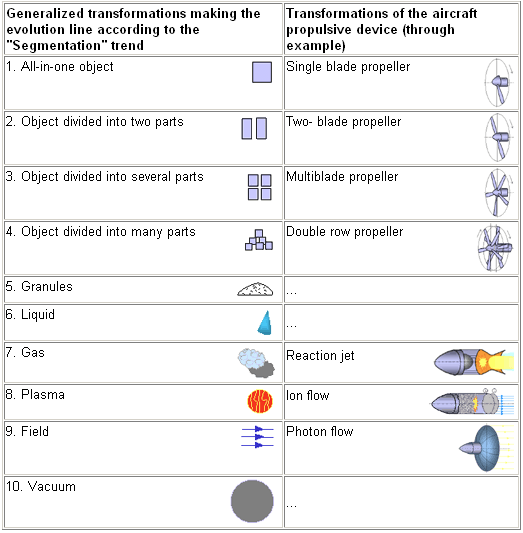
\includegraphics[width=0.75\linewidth]{figures/aircraft.png}
  \caption{\small Shpakovsky's evolution tree of the aircraft propulsion
    device \cite{Shpakovsky2003}}
	\label{fig:aircraft}
\end{figure*}

As a further example Shpakovsky provides is the evolution of the aircraft
propulsion device. Airplanes don't include sailplanes as it is stated that an
airplane must use an engine. This engine drives the propulsion device, in its
earliest form a propeller, which in turn moves the aircraft forward. The
elemental function of the object \textit{aircraft propulsion device} is
defined as \textit{A propulsive device is what an aircraft uses to push off
  the surrounding space while flying.} \cite{Shpakovsky2003}.

The starting point of the evolution is the single-bladed propeller, which
corresponds to the monolith in the segmentation pattern. Subsequently the two
parts transformation would be a double bladed propellers. The Evolution Tree
Trunk consists here of the entire tree as the object develops along the
segmentation pattern.

For granules, liquid and vacuum exists no current transformation. These gaps
can be used to theorise about potential inventions, cost and feasibility must
also be considered to get a good solution. While for example water can be
sprayed into the propeller area to increase the thrust, this can only be done
for short periods as water is expensive to carry all the time. Throwing away
rocket stages for further acceleration of a space craft are also proposed for
the granules transformation, but fuel tanks bear little resemblance to
granules. The granules, liquid and gas transformations are thus left empty on
the tree and are thus not modelled. 

The same way as described from before is used to model the evolution tree. An
example for adding an extra propeller row is provided below, the full version
can be seen in \textit{AircraftPropulsionDeviceExample.ttl}. 

\begin{code}\tt
ex:AircraftPropulsionDevice \\
\> a tc:SpecificEvolutionTree ; \\
\> skos:prefLabel "Propulsion device for aircraft"@en ; \\
\> skos:definition "A propulsive device is what an aircraft \\
\>\> uses to push off the surrounding space while flying"@en .\\[4pt]
ex:MultiBladePropeller \\
\> a ex:AircraftPropulsionDevice ; \\
\> ex:addPropellerRow ex:DoubleRowPropeller ; \\
\> skos:prefLabel "Multiblade propeller"@en .\\[4pt]
ex:addPropellerRow \\
\> a rdf:Property, skos:Concept ; \\
\> od:usesPattern tc:SegmentationPattern, tc:ManyParts ; \\
\> skos:prefLabel "Add propeller row"@en .
\end{code}

\begin{thebibliography}{xxx}
\raggedright
\bibitem{Altshuller1979} Genrich Altshuller (1979).  Creativity as an exact
  science (in Russian). English version: Gordon and Breach, New York 1988.
\bibitem{Graebe2021} Hans-Gert Gr\"abe (2021). The WUMM Project on a TRIZ
  Ontology. Basic Concepts.
  \url{https://wumm-project.github.io/Texts/WOP-Basics.pdf}.
\bibitem{KS} Karl Koltze, Valeri Souchkov (2017).  Systematische
  Innovationsmethoden (in German).  Hanser, Munich. ISBN 978-3-446-45127-8.
\bibitem{TESE2018} Alex Lyubomirsky, Simon Litvin, Sergei Ikovenko et al.
  (2018). Trends of Engineering System Evolution (TESE).  TRIZ Consulting
  Group. ISBN 9783000598463.
\bibitem{Shpakovsky2003} Nikolay Shpakovsky (2003). One of the evolution
  trends of an aircraft propulsive device.\\
  \url{http://www.gnrtr.com/Generator.html?pi=211&cp=3}
\bibitem{Shpakovsky2016} Nikolay Shpakovsky (2016). Tree of Technology
  Evolution. English translation of the Russian original (Forum, Moscow
  2010).\\ \url{https://wumm-project.github.io/TTS.html}
\bibitem{SKOS} SKOS -- The Simple Knowledge Organization System.
  \url{https://www.w3.org/TR/skos-reference/}.  
\bibitem{WUMM} The WUMM Project. \url{https://wumm-project.github.io/} 
\end{thebibliography}

\end{document}
